\documentclass{statsoc}
% \usepackage{mathtime}
\usepackage{ccfonts,eulervm}
\usepackage{tabularx}
\usepackage{xr}
\externaldocument{supplementary_material}
% ---------------------------------------------------------------------------------------------------------------------------------
% The statsoc style file is broken?
% I have copied this code straight from stack overflow
% https://tex.stackexchange.com/questions/351768/problem-with-statsoc-class-and-pdflatex
\usepackage{geometry}

\geometry{
  textwidth=33pc,
  textheight=\dimexpr48\baselineskip+\topskip\relax,
  marginparsep=11pt,
  marginparwidth=107pt,
  footnotesep=6.65pt,
  headheight=9pt,
  headsep=9pt,
  footskip=30pt,
}
% ---------------------------------------------------------------------------------------------------------------------------------

% \usepackage{natbib}
\bibliographystyle{chicago}

%% bibliography stuff -- this needs come before the preamble inclusion
\usepackage{enumitem}
\usepackage{etex,etoolbox}
\usepackage{hyperref}
\usepackage{fullpage}
\setlength{\marginparwidth}{2cm}
\usepackage{todonotes}
\usepackage{multirow}
\usepackage{booktabs}

\def\gc{\overset{\text{GC}}{\rightarrow}}  % Granger causality arrow
\def\ngc{\overset{\text{GC}}{\nrightarrow}}  % Negated Granger causality arrow
\def\pwgc{\overset{\text{PW}}{\rightarrow}}  % Pairwise Granger causality arrow
\def\npwgc{\overset{\text{PW}}{\nrightarrow}}  % Negated pairwise Granger causality arrow
\def\te{\overset{\mathcal{T}}{\rightarrow}}  % Transfer entropy arrow
\def\gcg{\mathcal{G}}  % Granger-causality graph
\def\gcge{\mathcal{E}}  % Graph edges
\def\VAR{\mathsf{VAR}}  % VAR(p) model
\def\B{\mathsf{B}}  % Filter B
\def\wtB{\widetilde{\B}}  % General filter B
\def\A{\mathsf{A}}  % Filter A
\def\H{\mathcal{H}}  % Hilbert space

\newcommand{\linE}[2]{\hat{\E}[#1\ |\ #2]}  % Linear projection
\newcommand{\linEerr}[2]{\xi[#1\ |\ #2]}  % Error of linear projection
\newcommand{\pa}[1]{pa(#1)}  % Parents of a node
\newcommand{\anc}[1]{\mathcal{A}(#1)}  % Ancestors of a node
\newcommand{\ancn}[2]{\mathcal{A}_{#1}(#2)}  % nth ancestors of a node
\newcommand{\gpn}[2]{gp_{#1}(#2)}  % nth generation grandparents
\newcommand{\wtalpha}[2]{\widetilde{\alpha}(#1, #2)}  % Some notation for lem:pwgc_anc
\newcommand{\dist}[2]{\mathsf{d}(#1, #2)}  % Distance between things
\newcommand{\gcgpath}[2]{#1 \rightarrow \cdots \rightarrow #2}  % A shorter path command

% \usepackage{fullpage}
\usepackage{framed}

% Figures
\usepackage{graphicx}
\usepackage{caption}  % This is not recommended?
\usepackage{subcaption}
% \usepackage{wrapfig}
% \usepackage{svg}

% Math packages, theorem definitions and numbering
\usepackage{amsmath}
\usepackage{amssymb}
% \usepackage{amsthm}
% \usepackage{mathrsfs} % Fancy scripted font
\usepackage{bm}  % Bold math

% Misc packages
\usepackage[linesnumbered, ruled, vlined]{algorithm2e}
\usepackage{algorithm2e} %{algorithm} environment
\usepackage{soul}  % \hl highlighting
\usepackage{color}
\usepackage{mathtools}  % For my \ceil function

% Theorems (with italics)
% \theoremstyle{plain}  % Style definition removes italics
\newtheorem{theorem}{Theorem}
\newtheorem{corollary}{Corollary}
\newtheorem{proposition}{Proposition}
\newtheorem{lemma}{Lemma}

% \theoremstyle{definition}
\newtheorem{remark}{Remark}
\newtheorem{definition}{Definition}
\newtheorem{example}{Example}
\newtheorem{assumption}{Assumption}

% Should I do this?  It makes cross references much easier,
% but is possibly extra complication.
% \counterwithin{theorem}{section}
% \counterwithin{corollary}{section}
% \counterwithin{proposition}{section}
% \counterwithin{lemma}{section}

% \counterwithin{remark}{section}
% \counterwithin{definition}{section}
% \counterwithin{example}{section}
% \counterwithin{assumptions}{section}

% keywords
\providecommand{\keywords}[1]{\textbf{\textit{Keywords---}} #1}

% General
\def\defeq{\overset{\Delta}{=}}  % Equal with triangle
\def\cl{\mathsf{cl\ }}  % Closure
\newcommand{\sgn}[1]{\mathsf{sgn}(#1)}  % sign function

% Calculus
\def\d{\mathsf{d}}  % Differential operator

% Functions
\def\ln{\mathsf{ln\ }}  % Natural logarithm
\DeclarePairedDelimiter{\ceil}{\lceil}{\rceil}  % Ceiling

% Probability
\def\H{\mathcal{H}}  % Hilbert space
\def\E{\mathbb{E}}  % Expectation
\def\Var{\text{Var}}  % Variance
\def\P{\mathbb{P}}  % Probability Measure
\def\F{\mathcal{F}}  % A sigma algebra
\def\sX{\mathcal{X}}  % Another sigma algebra
\def\KL{\mathbf{D}_{KL}}  % KL divergence
\def\bF{\mathbf{F}}  % Whole F-meas space

% Standard sets
\def\Z{\mathbb{Z}}  % Set of integers
\def\R{\mathbb{R}}  % Set of real numbers
\def\C{\mathbb{C}}  % Set of complex numbers
\def\N{\mathbb{N}}  % Set of natural numbers
\def\ball{\mathbb{B}}  % Open ball
\def\clball{\overline{\ball}}  % Closed ball

% Linear algebra
\def\rk{\mathsf{rk }}  % The rank
\def\tr{\mathsf{tr }}  % The trace
\def\T{\mathsf{T}}  % Transpose notation
\def\c{\mathsf{c}}  % complement
\def\dg{\mathsf{dg }}   %  Diagonal vector of a matrix
\def\Dg{\mathsf{Dg }}   %  Diagonal matrix from a vector
\def\ind{\mathbf{1}}  % Ones vector or indicator
\def\matvec{\textbf{vec}}  % Vector operator
\def\<{\langle}  % < Inner product
\def\>{\rangle}  % > Inner product
\newcommand{\inner}[2]{\langle #1, #2 \rangle}  % Inner product
\newcommand{\innerT}[2]{#1^\T #2}  % Inner product for finite vectors

\graphicspath{{../figures/}}

\title{Graph Topological Aspects of Granger Causal Network Learning}
\author[Author 1 {\it et al.}]{R. J. Kinnear}
\address{
  University of Waterloo,
  Waterloo,
  Canada.}
\email{Ryan@Kinnear.ca}

\author{R. R. Mazumdar}
\address{
  University of Waterloo,
  Waterloo,
  Canada.}

\begin{document}

\abstract{We study Granger-causality in the context of wide-sense
  stationary time series, where our focus is on the topological
  aspects of the underlying causality graph.  We establish sufficient
  conditions (in particular, we develop the notion of a ``strongly
  causal'' graph topology) under which the true causality graph can be
  recovered via pairwise causality testing alone, and provide examples
  from the gene regulatory network literature suggesting that our
  concept of a strongly causal graph may be applicable to this field.
  We implement and detail finite-sample heuristics derived from our
  theory, and establish through simulation the efficiency gains (both
  statistical and computational) which can be obtained (in comparison
  to LASSO-type algorithms) when structural assumptions are met.}

\keywords{causality graph, gene regulatory networks,
  Granger-causality, network learning, time series, vector
  autoregression}

\paragraph{Acknowledgement}

We acknowledge the support of the Natural Sciences and Engineering Research Council of Canada (NSERC), [funding reference number 518418-2018].  Cette recherche a été financée par le Conseil de recherches en sciences naturelles et en génie du Canada (CRSNG), [numéro de référence 518418-2018].

\section{Introduction and Review}
\label{sec:introduction}
In this paper we study the notion of Granger-causality
\cite{granger1969investigating} \cite{Granger1980329} as a means of
uncovering an underlying causal structure in multivariate time series.
Though the underlying causality graph cannot be observed directly,
it's it's presence is inferred as a latent structure among observed
time series data.  This notion is leveraged in a variety of
applications e.g. in Neuroscience as a means of recovering
interactions amongst brain regions \cite{bressler2011wiener},
\cite{anna_paper2008}, \cite{david2008identifying}; in the study of
the dependence and connectedness of financial institutions
\cite{NBERw16223}; gene expression networks \cite{Fujita2007},
\cite{methods_for_inferring_gene_regulatory_networks_from_time_series_expression_data},
\cite{grouped_graphical_granger_modelling_for_gene_expression_regulatory_networks_discovery},
\cite{discovering_graphical_Granger_causality_using_the_truncating_lasso_penalty};
and power system design \cite{Misyrlis2016450}, \cite{yuan2014root}.

Granger-causality can generally be formulated by searching for the
``best'' graph structure consistent with observed data, which is in
general an extremely challenging problem (i.e. it may be framed as a
best subset selection problem, see, \cite{hastie_bss_comp} for recent
improvements in BSS methods), moreover, the comparison of quality
between different structures, and hence the notion of ``best'' needs
qualification.  In applications where we are interested merely in
minimizing the mean squared error of a linear one-step-ahead
predictor, then we will be satisfied with an entirely dense graph of
connections, since each edge can only serve to reduce estimation
error.  However, since the number of edges scales quadratically in $n$
(the number of nodes) it becomes imperative to infer a sparse
causality graph for large systems, both to avoid overfitting observed
data, as well as to aid the interpretability of the results.

A fairly early approach to the problem in the context of large systems
is provided by \cite{bach2004learning}, where the authors apply a
local search heuristic to the Whittle likelihood with an AIC
penalization.  The local search heuristic is a common approach to
combinatorial optimization due to it's simplicity, but is liable to
get stuck in shallow local minima.

A second and wildly successful heuristic is the LASSO regularizer
\cite{tibshirani1996regression}, which can be understood as a natural
convex relaxation to penalizing the count of the non-zero edges.  The
LASSO enjoys fairly strong theoretical guarantees
\cite{wainwright2009sharp}, extending largely to the case of
stationary time series data with a sufficiently fast rate of
dependence decay \cite{basu2015} \cite{wong2016lasso}
\cite{autoregressive_process_modelling_via_the_lasso_procedure}, and
variations on the LASSO have been applied in a number of different
time series contexts as well as Granger-causality
\cite{DBLP:journals/corr/HallacPBL17} \cite{haufe2008sparse}
\cite{bolstad2011causal} \cite{he2013stationary}
\cite{grouped_graphical_granger_modelling_for_gene_expression_regulatory_networks_discovery}.
One of the key improvements to the original LASSO algorithm is the
adaptive (i.e. weighted) ``adaLASSO'' \cite{adaptive_lasso_zou2006},
for which oracle results (i.e. asymptotic support recovery) are
established under less restrictive conditions than for the vanilla
LASSO.

% We study a novel perspective on the problem by establishing conditions
% under which simple \textit{pairwise} Granger-causality tests are
% sufficient to recover the entire graph.  Without particular
% topological assumptions, pairwise testing naturally results in a large
% number of false positives \cite{tam2013gene_pwgc}.

In the context of time series data, sparsity assumptions remain
important, but there is significant additional structure that may
arise as a result of considering the topology of the underlying
Granger-causality graph.  The focus of this paper is to shed light on
some of these topological questions, in particular, we study a
particularly simple notion of graph topology which we term
``strongly causal'' and show that stationary times series whose
underlying causality graph has this structure satisfy natural
intuitive notions of ``information flow'' through the graph.
Moreover, we show that such graphs are perfectly recoverable with only
\textit{pairwise} Granger-causality tests, which would otherwise
suffer from serious confounding problems (see
e.g. \cite{tam2013gene_pwgc} for earlier work on pairwise testing).
Aside from being an interesting theoretical perspective, prior
assumptions about the underlying graph (similarly to sparsity
assumptions) can greatly improve upon the statistical power of
causality graph recovery algorithms when the assumptions are met.

In the case of gene expression networks, we show examples from the
literature which suggest our concept of a ``strongly causal graph''
topology may have application in this field (see Section
\ref{sec:strongly_causal_graphs}).

The principle contributions of this paper are as follows: firstly, in
section \ref{sec:theory} we study \textit{pairwise} Granger-causality
relations, providing novel theorems connecting the structure of the
causality graph to the pairwise ``causality flow'' in the system, as
well as an interpretation in terms of the graph topology of the
sparsity pattern of matrices arising in the Wold decomposition,
generalizing in some sense the notion of ``feedback-free'' processes
studied by \cite{caines1975feedback} in close connection with
Granger-causality.  We establish sufficient conditions (sections
\ref{sec:strongly_causal_graphs}, \ref{sec:persistent_systems}) under
which a fully conditional Granger-causality graph can be recovered
from pairwise tests alone (sec \ref{sec:pairwise_algorithm}).  We
report a summary of simulation results in \ref{sec:simulation}, with
additional results reported in the supplementary material
\ref{apx:simulation}.  Our simulation results establish that there is
significant potential for improvement over existing methods, and that
the graph-topological aspects of time series analysis are relevant for
both theory and practice.  Concluding remarks on further open problems
and extensions are provided in Section \ref{sec:conclusion}.  The
proofs of each proposition and theorem are also relegated to the
supplementary material, simple corollaries have proofs included in the
main text.

\section{Graph Topological Aspects of Granger-causality}
\label{sec:theory}
\subsection{Formal Setting}
Consider the space $L_2(\Omega)$, the usual Hilbert space of finite
variance random variables over a probability space
$(\Omega, \mathcal{F}, \mathbb{P})$ having inner product
$\inner{x}{y} = \E[xy]$.  We will work with a discrete time and
wide-sense stationary (WSS) $n$-dimensional vector valued process
$x(t)$ (with $t \in \Z$) where the $n$ elements take values in $L_2$.
We suppose that $x(t)$ has zero mean, $\E x(t) = 0$, and has
absolutely summable matrix valued covariance sequence
$R(\tau) \overset{\Delta}{=} \E x(t)x(t - \tau)^\T$, and an absolutely continuous
spectral density.

We will also work frequently with the spaces spanned by the values of
such a process

\begin{equation}
  \label{eq:hilbert_space_defn}
  \begin{aligned}
    \H_t^x &= \cl \{\sum_{\tau = 0}^p a_\tau^\T x(t - \tau)\ |\ a_\tau \in \R^n, p \in \N\} \subseteq L_2(\Omega)\\
    H_t^x &= \{a x(t)\ |\ a \in \R\} \subseteq L_2(\Omega),
  \end{aligned}
\end{equation}

where the closure is naturally in mean-square.  We will often omit the
superscript $x$ which should be clear from context.  Evidently these
spaces are separable, and as closed subspaces of a Hilbert space they
are themselves Hilbert.  We will denote the spaces generated in
analogous ways by particular components of $x$ as e.g.
$\H_t^{(i, j)}$, $\H_t^{i}$ or by all but a particular component as
$\H_t^{-j}$.

As a consequence of the Wold decomposition theorem (see
e.g. \cite{lindquist}), every WSS sequence has the moving average
$MA(\infty)$ representation

\begin{equation}
  \label{eqn:wold}
  x(t) = c(t) + \sum_{\tau = 0}^\infty A(\tau) v(t - \tau),
\end{equation}

where $c(t)$ is a purely deterministic sequence, $v(t)$ is an
uncorrelated sequence and $A(0) = I$.  We will assume that $c(t) = 0$.
Given our setup, this representation can be inverted to yield the
$\VAR(\infty)$ form

\begin{equation}
  \label{eqn:ar_representation}
  x(t) = \sum_{\tau = 1}^\infty B(\tau) x(t - \tau) + v(t).
\end{equation}

The equations (\ref{eqn:wold}), (\ref{eqn:ar_representation}) can be
represented as $x(t) = \A(z)v(t) = \B(z)x(t) + v(t)$ via the action
(convolution) of the operators (LTI filters)
$\A(z) \defeq \sum_{\tau = 0}^\infty A(\tau)z^{-\tau}$ and
$\B(z) \defeq \sum_{\tau = 1}^\infty B(\tau)z^{-\tau}$ where the
operator $z^{-1}$ is the back shift operator acting on
$\ell_2^n(\Omega, \mathcal{F}, \mathbb{P})$, that is:

\begin{equation}
  \label{eqn:filter_action}
  \B_{ij}(z)x_j(t) \defeq \sum_{\tau = 1}^\infty B_{ij}(\tau)x_j(t - \tau).
\end{equation}

Finally, we have the inversion formula

\begin{equation}
  \label{eqn:lsi_inversion}
  \A(z) = (I - \B(z))^{-1} = \sum_{k = 0}^\infty \B(z)^k.
\end{equation}

The aforementioned assumptions are quite weak.  The strongest
assumption we require is finally that $\Sigma_v$ is a diagonal
positive-definite matrix, which is referred to as a lack of
instantaneous feedback in $x(t)$.  We formally state our setup as a
definition, which is the setup for the remainder of the paper:

\begin{definition}[Basic Setup]
  \label{def:basic_setup}
  The process $x(t)$ is an $n$ dimensional wide sense stationary
  process having invertible $\VAR(\infty)$ representation
  \eqref{eqn:ar_representation} where $v(t)$ is sequentially
  uncorrelated and has a diagonal positive-definite covariance matrix.
  The $MA(\infty)$ representation of equation \eqref{eqn:wold} has
  $c(t) = 0$ and $A(0) = I$.
\end{definition}

\subsection{Granger Causality}

\begin{definition}[Granger Causality]
  \label{def:granger_causality}
  For the WSS series $x(t)$ satisfying the assumptions of Definition
  \ref{def:basic_setup} we will say that component $x_j$
  \textit{Granger-Causes} (GC) component $x_i$ (with respect to $x$)
  and write $x_j \gc x_i$ if

\begin{equation}
  \linEerr{x_i(t)}{\H_{t - 1}} < \linEerr{x_i(t)}{\H^{-j}_{t - 1}},
\end{equation}

where $\xi[x \ |\ \H] \defeq \E (x - \linE{x}{\H})^2$ is the mean
squared estimation error and $\linE{x}{\H} \defeq \text{proj}_{\H}(x)$
denotes the (unique) projection onto the Hilbert space $\H$.
\end{definition}

This notion captures the idea that the process $x_j$ provides
information about $x_i$ that is not available from elsewhere.  The
caveat ``with respect to $x$'' is important in that GC relations can
change when components are added to or removed from our collection $x$
of observations, e.g. new GC relations can arise if we remove the
observations of a common cause, and existing GC relations can
disappear if we observe a new mediating series. The notion is closely
related to the information theoretic measure of transfer entropy,
indeed, if the distribution of $v(t)$ is known to be Gaussian then
they are equivalent \cite{barnett2009granger}.

The notion of conditional orthogonality is the essence of
Granger-causality, and enables us to obtain results for a fairly
general class of WSS processes, rather than simply $\VAR(p)$ models.

\begin{definition}[Conditional Orthogonality]
  \label{lem:conditional_orthogonality_equivalence}
  Consider three closed subspaces of a Hilbert space $\mathcal{A}$,
  $\mathcal{B}$, $\mathcal{X}$.  We say that $\mathcal{A}$ is
  conditionally orthogonal to $\mathcal{B}$ given $\mathcal{X}$
  and write $\mathcal{A} \perp \mathcal{B}\ |\ \mathcal{X}$ if

    \begin{equation*}
      \inner{a - \linE{a}{\mathcal{X}}}{b - \linE{b}{\mathcal{X}}} = 0\ \forall a \in \mathcal{A}, b \in \mathcal{B}.
    \end{equation*}

  An equivalent condition is that (see \cite{lindquist} Proposition 2.4.2)
  \begin{equation*}
    \linE{\beta}{\mathcal{A} \vee \mathcal{X}} = \linE{\beta}{\mathcal{X}}\ \forall \beta \in \mathcal{B}
  \end{equation*}
\end{definition}

\begin{theorem}[Granger Causality Equivalences]
  \label{thm:granger_causality_equivalences}
  The following are equivalent:

  \begin{enumerate}
    \item{$x_j \ngc x_i$}
    \item{$\forall \tau \in \N_+\ B_{ij}(\tau) = 0$ i.e. $\B_{ij}(z) = 0$}
    \item{$H_t^{i} \perp \H_{t - 1}^{j}\ |\ \H_{t - 1}^{-j}$}
    \item{$\linE{x_i(t)}{\H_{t - 1}^{-j}} = \linE{x_i(t)}{\H_{t - 1}}$}
  \end{enumerate}
\end{theorem}

\subsection{Granger Causality Graphs}
We establish some graph theoretic notation and terminology, collected
formally in definitions for the reader's convenient reference.

\begin{definition}[Graph Theory Review]
  A \textit{graph} $\gcg = (V, \gcge)$ is simply a
  tuple of sets respectively called \textit{nodes} and \textit{edges}.
  Throughout this paper, we have in all cases
  $V = [n] \defeq \{1, 2, \ldots, n\}$.  We will also focus solely on
  \textit{directed} graphs, where the edges
  $\gcge \subseteq V \times V$ are \textit{ordered} pairs.

  A (directed) \textit{path} (of length $r$) from node $i$ to node
  $j$, denoted $\gcgpath{i}{j}$, is a sequence
  $a_0, a_1, \ldots, a_{r - 1}, a_r$ with $a_0 = i$ and $a_r = j$ such
  that $\forall\ 0 \le k \le r\ (a_k, a_{k + 1}) \in \gcge$, and where
  $(a_k, a_{k - 1})$ are \textit{distinct} for $0 \le k < r$.

  A \textit{cycle} is a path of length $2$ or more between a node and
  itself.  An edge between a node and itself $(i, i) \in \gcge$ (which
  we do not consider to be a cycle) is referred to as a \textit{loop}.

  A graph $\gcg$ is a \textit{directed acyclic graph} (DAG) if it is a
  directed graph and does not contain any cycles.
\end{definition}

\begin{definition}[Parents, Grandparents, Ancestors]
  A node $j$ is a \textit{parent} of node $i$ if $(j, i) \in \gcge$.
  The set of all $i$'s parents will be denoted $\pa{i}$, and we
  explicitly exclude loops as a special case, that is,
  $i \not\in \pa{i}$ even if $(i, i) \in \gcge$.

  The set of level $\ell$ \textit{grandparents} of node $i$, denoted
  $\gpn{\ell}{i}$, is the set such that $j \in \gpn{\ell}{i}$ if and
  only if there is a \textit{directed path} of length $\ell$ in $\gcg$
  from $j$ to $i$.  Clearly, $\pa{i} = \gpn{1}{i}$.

  Finally, the set of \textit{level $\ell$ ancestors} of $i$:
  $\ancn{\ell}{i} = \bigcup_{\lambda \le \ell}\gpn{\lambda}{i}$ is the
  set such that $j \in \ancn{\ell}{i}$ if and only if there is a
  directed path of length $\ell$ \textit{or less} in $\gcg$ from $j$
  to $i$.  The set of \textit{all ancestors} of $i$
  (i.e. $\ancn{n}{i}$) is denoted simply $\anc{i}$.

  Recall that we do not allow a node to be it's own parent, although
  unless $\gcg$ is a DAG, a node \textit{can} be it's own ancestor.
  We will occasionally need to explicitly exclude $i$ from $\anc{i}$,
  in which case we will write $\anc{i}\setminus \{i\}$.
\end{definition}

Our principle object of study will be a graph determined by
Granger-causality relations as follows.

\begin{definition}[Causality graph]
  We define the Granger-causality graph $\gcg = ([n], \gcge)$ to be the directed
  graph formed on $n$ vertices where an edge $(j, i) \in \gcge$ if and
  only if $x_j$ Granger-causes $x_i$ (with respect to $x$).  That is,
  $$(j, i) \in \gcge \iff j \in \pa{i} \iff x_j \gc x_i.$$
\end{definition}

The edges of the Granger-causality graph $\gcg$ can be given a general
notion of ``weight'' by associating an edge $(j, i)$ with the
\textit{strictly causal} LTI filter $\B_{ij}(z)$ (see eqn
\eqref{eqn:filter_action}).  Thence, the matrix $\B(z)$ is analogous
to a \textit{weighted adjacency matrix}\footnote{\footnotesize We are using the
  convention that $\B_{ij}(z)$ is a filter with input $x_j$ and output
  $x_i$ so as to write the action of the system as $\B(z)x(t)$ with
  $x(t)$ as a column vector.  This competes with the usual convention
  for adjacency matrices where $A_{ij} = 1$ if there is an edge
  $(i, j)$.  In our case, the sparsity pattern of $\B_{ij}$ is the
  \textit{transposed} conventional adjacency matrix.} for the graph $\gcg$.  And,
in the same way that the $k^{\text{th}}$ power of an adjacency matrix
counts the number of paths of length $k$ between nodes,
$(\B(z)^k)_{ij}$ is a filter isolating the ``action'' of $j$ on $i$ at
a time lag of $k$ steps, this is exemplified in the inversion formula
\ref{eqn:lsi_inversion}.

From the $\VAR$ representation of $x(t)$ there is clearly a tight
relationship between each node and it's parent nodes, the relationship
is quantified through the sparsity pattern of $B(z)$.  Similarly, the
following proposition is analogous to the definition of feedback free
processes of \cite{caines1975feedback} and provides an interpretation
of the sparsity pattern of $A(z)$ (from the MA representation of
$x(t)$) in terms of the causality graph $\gcg$.

\begin{proposition}[Ancestor Expansion]
  \label{prop:parent_expanding}
  The component $x_i(t)$ of $x(t)$ can be represented in terms of it's
  parents in $\gcg$:

  \begin{equation}
    \label{eqn:parent_expansion}
    x_i(t) = v_i(t) + \B_{ii}(z)x_i(t) + \sum_{k \in \pa{i}}\B_{ik}(z)x_k(t).
  \end{equation}

  Moreover, $x_i$ can be expanded in terms of it's ancestor's $v(t)$
  components only:

  \begin{equation}
    \label{eqn:ancestor_expansion}
    x_i(t) = \A_{ii}(z)v_i(t) + \sum_{\substack{k \in \anc{i} \\ k \ne i}}\A_{ik}(z)v_k(t),
  \end{equation}

  where $\A(z) = \sum_{\tau = 0}^\infty A(\tau)z^{-\tau}$ is the filter from
  the Wold decomposition representation of $x(t)$, equation
  (\ref{eqn:wold}).
\end{proposition}

This statement is ultimately about the sparsity pattern in the Wold
decomposition matrices $A(\tau)$ since
$x_i(t) = \sum_{\tau = 0}^\infty \sum_{j = 1}^n A_{ij}(\tau)v_j(t -
\tau)$.  The proposition states that if $j \not \in \anc{i}$ then
$\A_{ij}(z) = 0$.  

\subsection{Pairwise Granger Causality}
\label{sec:pwgc}
Recall that Granger-causality in general must be understood with
respect to a particular universe of observations.  If $x_j \gc x_i$
with respect to $x_{-k}$, it may not hold with respect to $x$.  For
example, $x_k$ may be a common ancestor which when observed, completely
explains the connection from $x_j$ to $x_i$.  In this section we study
\textit{pairwise} Granger-causality, and seek to understand when
knowledge of pairwise relations is sufficient to deduce the true fully
conditional relations of $\gcg$.

\begin{definition}[Pairwise Granger-causality]
  We will say that $x_j$ pairwise Granger-causes $x_i$ and write
  $x_j \pwgc x_i$ if $x_j$ Granger-causes $x_i$ with respect only to
  $(x_i, x_j)$.
\end{definition}

This notion is of interest for a variety of reasons.  From a purely
conceptual standpoint, we will see how the notion can in some sense
capture the idea of ``flow of information'' in the underlying graph,
in the sense that if $j \in \anc{i}$ we expect that $j \pwgc i$.  It may
also be useful for reasoning about the conditions under which
\textit{unobserved} components of $x(t)$ may or may not interfere with
inference in the actually observed components.  Finally, motivated
from a practical standpoint to analyze causation in large systems,
practical estimation procedures based purely on pairwise causality
tests are of interest since the computation of such pairwise relations
is substantially easier.

The following propositions are essentially lemmas used for the proof
of the upcoming Proposition \ref{prop:ancestor_properties}, but
remain relevant for providing intuitive insight into the problems at
hand.

\begin{proposition}
  Consider distinct nodes $i, j$ in a Granger-causality graph
  $\gcg$.  If

  \begin{enumerate}[label=(\alph*)]
    \item{$j \not\in \anc{i}$ and $i \not\in \anc{j}$}
    \item{$\anc{i}\cap\anc{j} = \emptyset$}
  \end{enumerate}

  then $\H_t^{(i)} \perp \H_t^{(j)}$, that is,
  $\forall s, \tau \in \Z_+\ \E[x_i(t - s)x_j(t - \tau)] = 0$.  Moreover,
  this means that $j \npwgc i$ and $\linE{x_j(t)}{\H_t^i} = 0$.
\end{proposition}

\begin{remark}
  The possibility that there exist nodes sharing both $i$ and $j$ as
  ancestors is not excluded, the point being that the temporal nature
  of Granger-causality eliminates the problems caused by ``colliders''
  (in the language of Pearl's causal calculus
  \cite{pearl2009causality}) in static causal inference.
\end{remark}

\begin{remark}
  It is possible for components of $x(t)$ to be correlated at some
  time lags without resulting in pairwise causality.  For instance,
  the conclusion $j \npwgc i$ of Proposition
  \ref{prop:separated_ancestor_uncorrelated} will still hold even if
  $i \in \anc{j}$, since $j$ cannot provide any information about $i$
  that is not available from observing $i$ itself.
  % However, it is important to note that this is the case only if we
  % have direct access to $x(t)$.  That is, if we instead observed a
  % noisy version of $x$ (i.e. $\tilde{x}(t) = x(t) + n(t)$) the
  % observation of $\tilde{x}_j$ would enable conditionally improved
  % estimates of $\tilde{x}_i$, without there necessarily being any
  % causal flow in the underlying system $x(t)$.
\end{remark}

\begin{proposition}
  Consider distinct nodes $i, j$ in a Granger-causality graph $\gcg$.
  If

  \begin{enumerate}[label=(\alph*)]
    \item{$j \not\in \anc{i}$}
    \item{$\anc{i}\cap\anc{j} = \emptyset$}
  \end{enumerate}

  then $j \npwgc i$.
\end{proposition}

The previous result can still be strengthened significantly; notice
that it is possible to have some $k \in \anc{i} \cap \anc{j}$ where still
$j \npwgc i$, an example is furnished by the three node graph
$k \rightarrow i \rightarrow j$ where clearly
$k \in \anc{i}\cap\anc{j}$ but $j \npwgc i$.  We must introduce the concept
of a \textit{confounding} variable, which effectively eliminates the
possibility presented in this example.

\begin{definition}[Confounder]
  A node $k$ will be referred to as a \textit{confounder} of nodes
  $i, j$ (neither of which are equal to $k$) if
  $k \in \anc{i} \cap \anc{j}$ and there exists a path
  $\gcgpath{k}{i}$ not containing $j$, and a path $\gcgpath{k}{j}$ not
  containing $i$. A simple example is furnished by the ``fork'' graph
  $i \leftarrow k \rightarrow j$.
\end{definition}

\begin{proposition}
  \label{prop:ancestor_properties}
  If in a Granger-causality graph $\gcg$ where $j \pwgc i$ then
  $j \in \anc{i}$ or $\exists k \in \anc{i} \cap\anc{j}$ which is a
  confounder of $(i, j)$.
\end{proposition}

\begin{remark}
  The interpretation of this proposition is that for $j \pwgc i$ then
  there must either be ``causal flow'' from $j$ to $i$
  ($j \in \anc{i}$) or there must be a confounder $k$ through which
  common information is received.
\end{remark}

An interesting corollary is the following:

\begin{corollary}
  If the graph $\gcg$ is a DAG then $j \pwgc i, i \pwgc j \implies \exists k \in \anc{i} \cap \anc{j}$ confounding $(i, j)$.
\end{corollary}

It seems reasonable to expect a converse of Proposition
\ref{prop:ancestor_properties} to hold, i.e.
$j \in \anc{i} \Rightarrow j \pwgc i$.  Unfortunately, this is not the
case in general, as different paths through $\gcg$ can lead to
cancellation (see Figure \ref{fig:diamond_cancellation}).  In fact, we
do not even have $j \in \pa{i} \Rightarrow j \pwgc i$ (see Figure
\ref{fig:lag_cancellation}).

\begin{example}
  \label{ex:diamond_cancellation}
  Firstly, on $n = 4$ nodes, ``diamond'' shapes can lead to cancellation on paths of length 2:

\begin{equation*}
  x(t) =
  \left[
    \begin{array}{cccc}
      0 & 0 & 0 & 0\\
      a & 0 & 0 & 0\\
      -a & 0 & 0 & 0\\
      0 & 1 & 1 & 0\\
    \end{array}
  \right] x(t - 1) + v(t),
\end{equation*}

with $\E v(t) = 0,\ \E v(t)v(t - \tau)^\T = \delta_\tau I$.

By directly calculating

\begin{align*}
  x_4(t) &= x_2(t - 1) + x_3(t - 1) + v_4(t)\\
         &= ax_1(t - 2) + av_2(t - 1) - ax_1(t - 2) -av_3(t - 1) + v_4(t)\\
         &= a(v_2(t - 1) - v_3(t - 1)) + v_4(t),
\end{align*}

we see that, since $v(t)$ is isotropic white noise, $1 \npwgc 4$.  The problem here is that there are multiple paths from $x_1$ to $x_4$.
\end{example}

\begin{figure}
  \centering
  \caption{Examples illustrating the difficulty of obtaining a converse to Proposition \ref{prop:ancestor_properties}}
  \begin{subfigure}[b]{0.35\textwidth}
    \includegraphics[width=\linewidth]{example1.pdf}
    \caption{Path cancellation: $j \in \anc{i} \nRightarrow j \pwgc i$}
    \label{fig:diamond_cancellation}
  \end{subfigure}
  \begin{subfigure}[b]{0.35\textwidth}
    \includegraphics[width=\linewidth]{example2.pdf}
    \caption{Cancellation from time lag: $j \in \pa{i} \nRightarrow j \pwgc i$}
    \label{fig:lag_cancellation}
  \end{subfigure}
\end{figure}

\begin{example}
  \label{ex:lag_cancellation}
  A second example on $n = 3$ nodes is also worth examining, in this case
  cancellation is a result of differing time lags.

\begin{equation*}
  x(t) =
  \left[
    \begin{array}{ccc}
      0 & 0 & 0\\
      -a & 0 & 0\\
      0 & 1 & 0\\
    \end{array}
  \right] x(t - 1) +
  \left[
    \begin{array}{ccc}
      0 & 0 & 0\\
      0 & 0 & 0\\
      a & 0 & 0\\
    \end{array}
  \right] x(t - 2) + v(t)
\end{equation*}

Then

\begin{align*}
  x_2(t) &= v_2(t) - ax_1(t - 1)\\
  x_3(t) &= v_3(t) + x_2(t - 1) + ax_1(t - 2)\\
  \Rightarrow x_3(t) &= v_2(t - 1) + v_3(t),
\end{align*}

and again $1 \npwgc 3$.
\end{example}

\subsection{Strongly Causal Graphs}
\label{sec:strongly_causal_graphs}

In this section and the next we will seek to understand when converse
statements of Proposition \ref{prop:ancestor_properties} \textit{do}
hold.  One possibility is to restrict the coefficients of the system
matrix, e.g. by requiring that $B_{ij}(\tau) \ge 0$.  Instead,
we think it more meaningful to focus on the defining feature of
time series networks, that is, the topology of $\gcg$.

\begin{definition}[Strongly Causal]
  \label{def:strongly_causal}
  We will say that a Granger-causality graph $\gcg$ is
  \textit{strongly causal} if there is at most one directed path between
  any two nodes.  Strongly Causal Graphs will be referred to as SCGs.
\end{definition}

Examples of strongly causal graphs include directed trees (or
forests), DAGs where each node has at most one parent, and Figure
\ref{fig:example_fig3} of this paper.  A complete bipartite graph with
$2n$ nodes is also strongly causal, demonstrating that the number of
edges of such a graph can still scale quadratically with the number of
nodes.  It is evident that the strong causal property is inherited by
subgraphs.

\begin{example}
  Though examples of SCGs are easy to construct in theory, should
  practitioners expect SCGs to arise in application?  While a positive
  answer to this question is not \textit{necessary} for the concept to
  be useful, it is certainly sufficient.  Though the answer is likely
  to depend upon the particular application area, examples appear to
  be available in biology, in particular, the authors of
  \cite{discovering_graphical_Granger_causality_using_the_truncating_lasso_penalty}
  cite an example of the so called ``transcription regulatory network
  of \textit{E.coli}'', and
  \cite{learning_genome_scale_regulatory_networks} study a much larger
  regulatory network of \textit{Saccharomyces cerevisiae}.  These
  networks, which we reproduce in Figure \ref{fig:gene_networks},
  appear to have at most a small number of edges which violate the
  strong-causality condition.

  \begin{figure}[h]
    \centering
    \caption{Transcription Regulatory Networks}
    \label{fig:gene_networks}
    \begin{subfigure}[b]{0.45\textwidth}
      \caption{\textit{E.Coli} Network of
        \cite{discovering_graphical_Granger_causality_using_the_truncating_lasso_penalty}}
      \label{fig:gene_network1}
      \includegraphics[width=\linewidth, height=\linewidth]{ecoli_regulatory_network.png}
    \end{subfigure}
    \begin{subfigure}[b]{0.45\textwidth}
      \caption{\textit{Saccharomyces cerevisiae} Network of
        \cite{learning_genome_scale_regulatory_networks}}
      \label{fig:gene_network2}
      \includegraphics[width=\linewidth, height=\linewidth]{huge_gene_network.png}
    \end{subfigure}

    {\footnotesize Figure \ref{fig:gene_network1} has only one edge
      violating the strong-causality assumption, and Figure
      \ref{fig:gene_network2} appears qualitatively to be nearly
      strongly causal.  In particular, most of the edges are emanating
      from network hubs, and many of the other edges are colliders.

      Figure \ref{fig:gene_network1}
      is reproduced under the Creative Commons Attribution
      Non-Commercial License
      (http://creativecommons.org/licenses/by-nc/2.5) and Figure
      \ref{fig:gene_network2} under the Creative Commons Attribution
      License (https://creativecommons.org/licenses/by/4.0/)}
  \end{figure}
\end{example}

For later use, and to get a feel for the topological implications of
strong causality, we explore a number of properties of such graphs
before moving into the main result of this section.  The following
important property essentially strengthens Proposition
\ref{prop:ancestor_properties} for the case of strongly causal graphs.

\begin{proposition}
  \label{prop:sc_graph_common_anc}
  In a strongly causal graph if $j \in \anc{i}$ then any
  $k \in \anc{i} \cap \anc{j}$ is not a confounder, that is,
  the unique path from $k$ to $i$ contains $j$.
\end{proposition}

\begin{corollary}
  \label{cor:parent_corollary}
  If $\gcg$ is a strongly causal DAG then $i \pwgc j$ and $j \in \anc{i}$ are
  \textit{alternatives}, that is $i \pwgc j \Rightarrow j \notin \anc{i}$.
\end{corollary}
\begin{proof}
  Suppose that $i \pwgc j$ and $j \in \anc{i}$.  Then since $\gcg$ is
  acyclic $i \not\in \anc{j}$, and by Proposition
  \ref{prop:ancestor_properties} there is some
  $k \in \anc{i}\cap\anc{j}$ which is a confounder.  However, by
  Proposition \ref{prop:sc_graph_common_anc} $k$ cannot be a
  confounder, a contradiction.
\end{proof}
% This is a direct proof
  % \begin{proof}
%   Suppose that $\gcg$ is a strongly causal DAG and that we have both
%   $i \pwgc j$ and $j \in \anc{i}$, which implies that
%   $i \not \in \anc{j}$ since $\gcg$ is a DAG.  We will establish the
%   contradiction $i \in \anc{j}$.

%   Since $j \in \anc{i}$ there is a path $\gcgpath{j}{i}$.
%   Moreover, since $i \pwgc j$ by Proposition \ref{prop:pwgc_anc} there
%   must be a confounding ancestor $k \in \anc{i} \cap \anc{j}$, where the
%   node $k$ has a path to $j,\ \gcgpath{k}{j}$, as well as a path
%   to $i,\ \gcgpath{k}{i}$.

%   \hl{Double check that the ancestor properties Proposition implies
%     that BOTH paths do not contain the other node.}

%   Now, since the graph is strongly causal, the only possible
%   $\gcgpath{k}{i}$ path is the one obtained by concatenating the
%   $\gcgpath{k}{j}$ path with the $\gcgpath{j}{i}$ path.
%   However, this is a contradiction since $k$ is a confounder and
%   should have a $\gcgpath{k}{i}$ path which does not contain $i$.
% \end{proof}
  
\begin{corollary}
  \label{cor:bidirectional_edge}
  If $\gcg$ is a strongly causal DAG such that $i \pwgc j$ and
  $j \pwgc i$, then $i \not\in \anc{j}$ and $j \not\in \anc{i}$.  In
  particular, a pairwise bidirectional edge indicates the absence of
  any edge in $\gcg$.
\end{corollary}
\begin{proof}
  This follows directly from applying Corollary
  \ref{cor:parent_corollary} to $i \pwgc j$ and $j \pwgc i$.
% This is a direct proof
% \begin{proof}
  % By way of contradiction, suppose that $i \in \pa{j}$.  We will
  % consider the two possibilities allowed by proposition
  % \ref{prop:ancestor_properties} for $j \pwgc i$.  Firstly
  % $j \in \anc{i}$ is impossible since $\gcg$ is assumed to be acyclic.
  % Secondly, if there is some confounding node
  % $u \in \anc{i} \cap \anc{j}$ with a path
  % $u \rightarrow \cdots \rightarrow j$ which does not contain $i$ we
  % have a contradiction since there must now be multiple
  % $u \rightarrow j$ paths: the aforementioned, and a path
  % $u \rightarrow \cdots \rightarrow i \rightarrow \cdots \rightarrow
  % j$ which \textit{does} contain $i$.  We conclude that $i \in \pa{j}$
  % is impossible, and symmetrically that $j \in \pa{i}$ is as well.
% \end{proof}
\end{proof}

In light of Proposition \ref{prop:sc_graph_common_anc}, the following
provides a partial converse to Proposition
\ref{prop:ancestor_properties}, and supports the intuition of ``causal
flow'' through paths in $\gcg$.

\begin{proposition}
  \label{prop:pwgc_anc}
  If $\gcg$ is a strongly causal DAG then $j \in \anc{i} \Rightarrow j \pwgc i$.
\end{proposition}

We immediately obtain the corollary, which we remind the reader is,
surprisingly, not true in a general graph.

\begin{corollary}
  \label{cor:gc_implies_pwgc}
  If $\gcg$ is a strongly causal DAG then $j \gc i \Rightarrow j \pwgc i$.
\end{corollary}

\begin{remark}
  As we have seen and as is true in much of statistics, confounding
  nodes pose challenges for Granger-causality.  However, as opposed to
  the causal calculus of \cite{pearl2009causality}, pairwise
  Granger-causality does not suffer any difficulty with so-called
  ``colliders'', that is, the topology $i \rightarrow k \leftarrow j$ will never result
  in $i \pwgc j$ or $j \pwgc i$.  This is evidently an advantage of
  the \textit{temporal} nature of Granger-causality -- there is no
  backwards causal flow along the edges of $\gcg$.
\end{remark}

\begin{example}
  As a final remark of this subsection we note that a complete
  converse to Proposition \ref{prop:ancestor_properties} is not
  possible without additional conditions.  Consider the ``fork''
  system on $3$ nodes (i.e. $2 \leftarrow 1 \rightarrow 3$) defined by

  \begin{equation*}
    x(t) =
    \left[
      \begin{array}{cccc}
        0 & 0 & 0\\
        a & 0 & 0\\
        a & 0 & 0\\
      \end{array}
    \right] x(t - 1) + v(t).
  \end{equation*}

  In this case, node $1$ is a confounder for nodes $2$ and $3$, but
  $x_3(t) = v_3(t) - v_2(t) + x_2(t)$ and $2 \npwgc 3$ (even
  though $x_2(t)$ and $x_3(t)$ are contemporaneously correlated)

  If we were to augment this system by simply adding an autoregressive
  component (i.e. some ``memory'') to $x_1(t)$ e.g.
  $x_1(t) = v_1(t) + b x_1(t - 1)$ then we \textit{would} have
  $2 \pwgc 3$ since then
  $x_3(t) = v_3(t) + av_1(t - 1) - bv_2(t - 1) + bx_2(t - 1)$.  We
  develop this idea further in the next section.
\end{example}

\subsection{Persistent Systems}
\label{sec:persistent_systems}
In section \ref{sec:strongly_causal_graphs} we obtained a converse to
part $(a)$ of Proposition \ref{prop:ancestor_properties} via the
notion of a strongly causal graph topology (see Proposition
\ref{prop:pwgc_anc}).  In this section, we study conditions under
which a converse to part $(b)$ will hold.

\begin{definition}[Lag Function]
  Given a causal filter $\B(z) = \sum_{\tau = 0}^\infty b(\tau)z^{-\tau}$
  define 

  \begin{align}
    \tau_0(\B) &= \text{inf }\{\tau \in \Z_+\ |\ b(\tau) \ne 0\},\\
    \tau_{\infty}(\B) &= \text{sup }\{\tau \in \Z_+\ |\ b(\tau) \ne 0\}.\\
  \end{align}

  i.e. the ``first'' and ``last'' coefficients of the filter $\B(z)$,
  where $\tau_\infty(\B) \defeq \infty$ if the filter has an infinite
  length, and $\tau_0(\B) \defeq \infty$ if $\B(z) = 0$.
\end{definition}

\begin{definition}[Persistent]
  We will say that the process $x(t)$ with Granger-causality graph
  $\gcg$ is \textit{persistent} if for every $i \in [n]$ and every
  $k \in \anc{i}$ we have $\tau_0(\A_{ik}) < \infty$ and $\tau_\infty(\A_{ik}) = \infty$.
\end{definition}

\begin{remark}
  In the context of Granger-causality, ``most'' systems should be
  persistent.  In particular, $\mathsf{\VAR}(p)$ models are likely to
  be persistent since these naturally result in an equivalent
  $\mathsf{MA}(\infty)$ representation, see Example
  \ref{ex:persistent_system}.

  Moreover, persistence is not the weakest condition necessary for the
  results of this section, the condition that for each $i, j$ there is
  some $k \in \anc{i}\cap\anc{j}$ such that
  $\tau_0(\A_{jk}) < \tau_\infty(\A_{ik})$ is enough.  The intuition
  being that nodes $i$ and $j$ are not receiving temporally disjoint
  information from $k$.

  The etymology for the persistence condition can be explained by
  supposing that the two nodes $i, j$ each have a loop (i.e.
  $\B_{ii}(z) \ne 0, \B_{jj}(z) \ne 0$) then this autoregressive
  component acts as ``memory'', and so the influence from the
  confounder $k$ \textit{persists} in $x_i(t)$, and
  $\tau_\infty(\A_{ik}) = \infty$ for each confounder is expected.
\end{remark}

\begin{example}
  \label{ex:persistent_system}
  Consider a process $x(t)$ generated by the $\VAR(1)$
  model\footnote{Recall that any $\VAR(p)$ model with $p < \infty$ can
    be written as a $\VAR(1)$ model, so we lose little generality in
    considering this case.}  having $\B(z) = Bz^{-1}$.  If $B$ is
  diagonalizable, and has at least $2$ distinct eigenvalues, then
  $x(t)$ is persistent.

  See the supplementary material for an analysis of this example.
\end{example}

In order to eliminate the possibility of a particular sort of
cancellation, an ad-hoc assumption is required.  Strictly speaking,
the persistence condition is not a necessary or sufficient condition
for the following, but cases where the following fails to hold, and
peristence \textit{does} hold, are unavoidable pathologies.

\begin{assumption}[no-cancellation]
  \label{ass:T_causality}
  Fix $i, j \in [n]$ and let $H_i(z)$ be the strictly-causal filter
  such that

  \begin{equation*}
    H_i(z)x_i(t) = \linE{x_i(t)}{\H_{t - 1}^i},
  \end{equation*}

  and similarly for $H_j(z)$.  Then define

  \begin{equation}
    \label{eqn:T_filter}
    T_{ij}(z) = \sum_{k \in \anc{i} \cap \anc{j}}\sigma_k^2\A_{ik}(z^{-1})(1 - H_i(z^{-1}))(1 - H_j(z))\A_{jk}(z),
  \end{equation}

  where $\sigma_k^2 = \E v_k(t)^2$.

  We will say that Assumption \ref{ass:T_causality} is satisfied if
  for every $i, j \in [n]$, $T_{ij}(z)$ is either constant over $z$
  (i.e. each $z^k$ coefficient for $k \in \Z \setminus \{0\}$ is $0$),
  or is \textit{neither} causal (i.e. containing only $z^{-k}$ terms,
  for $k \ge 0$) \textit{or} anti-causal (i.e. containing only $z^k$
  terms, for $k \ge 0$).  Put succinctly, $T_{ij}(z)$ must be
  two-sided.
\end{assumption}

\begin{remark}
  Under the condition of persistence, the only way for Assumption
  \ref{ass:T_causality} to fail is through cancellation in the terms
  defining $T_{ij}(z)$.  For example, the condition is assured if
  $x(t)$ is persistent, and there is only a single confounder.
  Unfortunately, some pathological behaviour resulting from
  confounding nodes seems to be unavoidable without some assumptions
  about the parameters of the $MA(\infty)$ system defining $x(t)$.
\end{remark}

\begin{proposition}
  \label{prop:persistence_converse}
  Fix $i, j \in [n]$ and suppose $\exists k \in \anc{i} \cap \anc{j}$
  which confounds $i, j$.  Then, if $T_{ij}(z)$ is not causal we have
  $j \pwgc i$, and if $T_{ij}(z)$ is not anti-causal we have
  $i \pwgc j$.  Moreover, if Assumption \ref{ass:T_causality} is
  satisfied, then $j \pwgc i \iff i \pwgc j$.
  % Suppose that Assumption \ref{ass:T_causality} is satisfied.  Then if
  % there exists a $k$ which confounds $(i, j)$ we have
  % $i \pwgc j \implies j \pwgc i$.  Moreover, if $T_{ij}(z)$ is not
  % constant, then $i \pwgc j$.
\end{proposition}

\begin{remark}
  The importance of this result is that when $i \pwgc j$ is a result
  of a condounder $k$, then $i \pwgc j \iff j \pwgc i$.  This
  implies that in a strongly causal graph every bidirectional pairwise
  causality relation must be the result of a confounder.  Therefore,
  in a strongly causal graph, pairwise causality analysis is
  \textit{immune to confounding} (since we can safely remove all
  bidrectional edges).
\end{remark}

\subsection{Recovering $\gcg$ via Pairwise Tests}
\label{sec:pairwise_algorithm}
We arrive at the main conclusion of the theoretical analysis in this
paper.

\begin{theorem}[Pairwise Recovery]
  \label{thm:scg_recovery}
  If the Granger-causality graph $\gcg$ for the process $x(t)$ is a
  strongly causal DAG and Assumption \ref{ass:T_causality} holds, then
  $\gcg$ can be inferred from pairwise causality tests.  The procedure
  can be carried out, assuming we have an oracle for pairwise
  causality, via Algorithm (\ref{alg:pwgr}).
\end{theorem}

\begin{algorithm}
  \SetKwInOut{Input}{input}
  \SetKwInOut{Output}{output}
  \SetKwInOut{Initialize}{initialize}
  \DontPrintSemicolon

  % \BlankLine
  \caption{Pairwise Granger Causality Algorithm}
  \label{alg:pwgr}
  \TitleOfAlgo{Pairwise Graph Recovery}
  \Input{Pairwise Granger-causality relations between a persistent
  process of dimension $n$ whose joint Granger-causality
  relations are known to form a strongly causal DAG $\gcg$.}
  % \Input{Pairwise Granger-causality relations}
  \Output{Edges $\gcge = \{(i, j) \in [n] \times [n]\ |\ i \gc j \}$ of
    the graph $\gcg$.}
  \Initialize{$S_0 = [n]$  \texttt{\# unprocessed nodes}\\
    $E_0 = \emptyset$  \texttt{\# edges of }$\gcg$\\
    % $P_0 = \emptyset$  \texttt{\# layer by layer driving nodes}\\
    $k = 1$ \texttt{\# a counter used only for notation}}
  \BlankLine
  $W \leftarrow \{(i, j)\ |\ i \pwgc j, j \npwgc i\}$  \texttt{\# candidate edges}\\
  $P_0 \leftarrow \{i \in S_0\ |\ \forall s \in S_0\ (s, i) \not\in W\}$  \texttt{\# parent-less nodes}\\
  \While{$S_{k - 1} \ne \emptyset$}{
    $S_k \leftarrow S_{k - 1} \setminus P_{k - 1}$ \texttt{\# remove nodes with depth }$k - 1$\\
    $P_k \leftarrow \{i \in S_k\ |\ \forall s \in S_k\ (s, i) \not\in W\}$   \texttt{\# candidate children}\\

    $D_{k0} \leftarrow \emptyset$\\
    \For{$r = 1, \ldots, k$} 
    {
      $Q \leftarrow E_{k - 1} \cup \big(\bigcup_{\ell = 0}^{r - 1} D_{k\ell}\big)$ \texttt{\# currently known edges}\\
      $D_{kr} \leftarrow \{(i, j) \in P_{k - r} \times P_k\ |\ (i, j) \in W,\ \text{no } i \rightarrow j \text{ path in } Q\}$
      % $E_k \leftarrow E_{k - 1} \cup D_{kr}$ \texttt{\# add edges to }$E_k$ \label{alg:inner_loop_end}\\
      % $W_{k + 1} \leftarrow W_k \setminus D_{kr}$  \texttt{\# remove edges from consideration}\\
    }
    $E_k \leftarrow E_{k - 1} \cup \big(\bigcup_{r = 1}^k D_{kr}\big)$ \texttt{\# update } $E_k$ \texttt{ with new edges}\\
    % \label{alg_line:inner_loop_end}\\
    % $W_{k + 1} \leftarrow W_k \setminus \big(\bigcup_{r = 0}^k D_{kr}\big)$  \texttt{\# remove edges from consideration}\\
    $k \leftarrow k + 1$
  }
  \Return{$E_{k - 1}$}
\end{algorithm}

The theorem is proven in the supplementary material by establishing
the correctness of Algorithm (\ref{alg:pwgr}).  The idea is to
iteratively ``peel away layers'' of nodes by removing the nodes that
have no parents remaining.  The requirement of strong causality
ensures that all actual edges of $\gcg$ manifest in some way as
pairwise relations (by Proposition \ref{prop:pwgc_anc}), and the
no-cancellation condition of Assumption \ref{ass:T_causality} allows
confounding to be eliminated by removing bidirectional edges (by
Proposition \ref{prop:persistence_converse} and Corollary
\ref{cor:bidirectional_edge}).  Without Assumption
\ref{ass:T_causality}, then each confounded pair would give rise to
$4$ possible pairwise topologies consistent with $\gcg$, one for each
type of pairwise edge (no edge, unidirectional, bidirectional).

\begin{example}
  The set $W$ collects ancestor relations in $\gcg$ (see Lemma
  \ref{lem:W_subset_E}).  In reference to Figure
  \ref{fig:example_fig3}, each of the solid black edges, as well as
  the dotted red edges will be included in $W$, but \textit{not} the
  bidirectional green dash-dotted edges, which we are able to exclude
  as results of confounding.  The groupings $P_0, \ldots, P_3$ are also
  indicated in Figure \ref{fig:example_fig3}.

  The algorithm proceeds first with the parent-less nodes $1, 2$ on the
  initial iteration where the edge $(1, 3)$ is added to $E$.  On the
  next iteration, the edges $(3, 4), (2, 4), (3, 5)$ are added, and
  the false edges $(1, 4), (1, 5)$ are excluded due to the paths
  $1 \rightarrow 3 \rightarrow 4$ and $1 \rightarrow 3 \rightarrow 5$
  already being present.  Finally, edge $(4, 6)$ is added, and the false
  $(1, 6), (3, 6), (2, 6)$ edges are similarly excluded due to the
  ordering of the inner loop.
  
  \begin{figure}
    \centering
    \caption{Example graph for Algorithm \ref{alg:pwgr}}
    {\footnotesize{Black arrows indicate true parent-child
        relations.  Red dotted arrows indicate pairwise causality (due to
        non-parent relations), green dash-dotted arrows indicate
        bidirectional pairwise causality (due to the confounding node
        $1$).  Blue groupings indicate each $P_k$ in Algorithm
        \ref{alg:pwgr}.}}
    \label{fig:example_fig3}
    
    \begin{subfigure}[b]{0.45\textwidth}
      \includegraphics[width=\linewidth]{example_algorithm.pdf}
    \end{subfigure}
    \begin{subfigure}[b]{0.45\textwidth}
      \includegraphics[width=\linewidth]{example_algorithm2.pdf}
    \end{subfigure}
  \end{figure}

  That we need to proceed backwards through $P_{k - r}$ as in the
  inner loop on $r$ can also be seen from this example, where if
  instead we simply added the set

  \begin{equation*}
    D_k' = \{(i, j) \in \Big(\bigcup_{r = 1}^k P_{k - r}\Big) \times P_k\ |\ i \pwgc j \}
  \end{equation*}

  to $E_k$ then we would infer the false positive edge
  $1 \rightarrow 4$.  Moreover, the same example shows that simply
  using the set

  \begin{equation*}
    D_k'' = \{(i, j) \in P_{k - 1} \times P_k\ |\ i \pwgc j \}  ,
  \end{equation*}

  causes the edge $1 \rightarrow 3$ to be missed.
\end{example}

% \begin{example}
%   We close this section by noting that the conditions of persistence
%   and strong causality are only sufficient conditions.  For example,
%   the complete directed graph with 2 nodes i.e.

%   \begin{equation*}
%     B(1) = \left[ \begin{array}{cc} 1/2 & 1 \\ 1 & 1/2 \end{array}\right]
%   \end{equation*}

%   contains a loop but is pairwise recoverable, though not by algorithm
%   (\ref{alg:pwgr}).  Clearly, this example is somewhat artificial
%   since when $n = 2$ there is no difference between pairwise
%   Granger-causality and joint Granger-causality amongst all series --
%   however, one can add any number of nodes having no parents or
%   children to a graph containing a length 2 cycle, in which case the
%   graph clearly remains pairwise recoverable.
% \end{example}

\section{Simulation}
\label{sec:simulation}
We implement an heuristic inspired by Algorithm \ref{alg:pwgr} by
replacing the population statistics with finite sample tests, the
details of which can be found in the supplementary material Section
\ref{sec:finite_pwgc} (see Algorithm \ref{alg:finite_pwgc}).  The
heuristic is essentially controlling the false discovery rate
substantially below what it would be with a threshold based pairwise
scheme.  The methods are easily parallelizable, and can scale to
graphs with thousands of nodes on a single machine.  By contrast,
scaling the LASSO to this large of a network (millions of variables)
is nontrivial and extremely computationally demanding.

We run experiments using two separate graph topologies having $n = 50$
nodes: a strongly causal graph (SCG) and a directed acyclic graph
(DAG).  Consult Section \ref{apx:simulation} for details on how data
is generated from these models.

We compare our results against the adaptive LASSO
\cite{adaptive_lasso_zou2006}, which outperformed both the LASSO and
the grouped LASSO by a large margin.  Motivated by scaling, we split the squared error
term into separate terms, one for each group of incident edges on a
node, and estimate the collection of $n$ incident filters
$\big\{\B_{ij}(z)\big\}_{j = 1}^n$ that minimizes
$\xi_i^{\text{LASSO}}$ in the following:

\begin{equation}
  \begin{aligned}
  \xi_i^{\text{LASSO}}(\lambda) &= \underset{B}{\text{min}}\ \frac{1}{T}\sum_{t = p_{\text{max}} + 1}^T\big(x_i(t) - \sum_{\tau = 1}^{p_{\text{max}}}\sum_{j = 1}^n B_{i, j}(\tau) x(t - \tau)\big)^2 + \lambda \sum_{\tau = 1}^{p_{\text{max}}} \sum_{j = 1}^n |B_{ij}(\tau)|\\
  \xi_i^{\text{LASSO}} &= \underset{\lambda \ge 0}{\text{min}}\ \xi_i^{\text{LASSO}}(\lambda) + \mathsf{BIC}\big(B_i^{\text{LASSO}}(\lambda)\big)\\
  \end{aligned}
\end{equation}

where we are choosing $\lambda$, the regularization parameters, via the BIC.
This is similar to the work of \cite{arnold2007temporal}, except that
we have replacing the LASSO with the Adaptive LASSO, which provides
dramatically superior performance.

\begin{figure}
  \centering
  \caption{Representative Random Graph Topologies on $n = 50$ Nodes}
  \label{fig:random_graph_topologies}
  \begin{subfigure}[b]{0.3\textwidth}
    \caption{SCG}
    \includegraphics[width=\linewidth]{example_scg.pdf}
  \end{subfigure}
  \begin{subfigure}[b]{0.3\textwidth}
    \caption{DAG $(q = \frac{2}{n})$}
    \includegraphics[width=\linewidth]{example_dag.pdf}
  \end{subfigure}
  \begin{subfigure}[b]{0.3\textwidth}
    \caption{DAG $(q = \frac{4}{n})$}
    \includegraphics[width=\linewidth]{example_dag_q.pdf}
  \end{subfigure}
\end{figure}

\begin{remark}[Graph Topologies]
  We depict in Figure \ref{fig:random_graph_topologies} the topologies
  of random graphs used in our empirical evaluation.  For values of
  $q$ close to $\frac{2}{n}$, the resulting random graphs tend to have
  a topology which is, at least qualitatively, close to the SCG.  As
  the value of $q$ increases, the random graphs deviate farther from
  the SCG topology, and we therefore expect the LASSO to outperform
  PWGC for larger values of $q$.
\end{remark}

\begin{remark}[MCC as a Support Recovery Measurement]
  We apply Matthew's Correlation Coefficient (MCC)
  \cite{matthews1975comparison} as a statistic for measuring support
  recovery performance.  This statistic synthesizes the confusion
  matrix into a single score appropriate for unbalanced labels and is
  calibrated to fall into the range $[-1, 1]$ with $1$ being perfect
  performance, $0$ being the performance of random guessing, and $-1$
  being perfectly opposed.
\end{remark}

\begin{remark}[Error Measurement]
  We estimate the 1-step ahead prediction error by forming the variance matrix estimate

  \begin{equation*}
    \widehat{\Sigma}_v \defeq \frac{1}{T_{\text{out}}} \sum_{t = 1}^{T_{\text{out}}} (x(t) - \widehat{x}(t))(x(t) - \widehat{x}(t))^\T
  \end{equation*}

  on a long stream of out-of-sample data.  We then report the quantity

  \begin{equation*}
    \frac{\ln \tr \widehat{\Sigma}_v}{\ln \tr \Sigma_v}
  \end{equation*}

  where $\widehat{\Sigma}_v = \Sigma_v$ is the best possible performance.
\end{remark}

\subsection{Results}
\begin{figure}[!h]
  \centering
  \caption{Simulation Results: PWGC vs AdaLASSO}
  \label{tab:simulation_table}

  \begin{tabular}{|ll||ll|ll|ll|}
    \toprule
    &\textbf{Algorithm}&alasso&pwgc&alasso&pwgc&alasso&pwgc\\
    &\textbf{Metric}&LRE&&FDP&&MCC&\\
    \textbf{T}&\textbf{q}&&&&&&\\
    \midrule
    \multirow{4}{*}{\textbf{50}}
    &\textbf{SCG}&1.71&\textbf{1.55}&0.52&\textbf{0.08}&0.46&\textbf{0.55}\\
    &\textbf{0.04}&1.97&\textbf{1.77}&0.57&\textbf{0.10}&0.41&\textbf{0.53}\\
    &\textbf{0.08}&2.95&\textbf{2.72}&0.50&\textbf{0.23}&0.36&\textbf{0.39}\\
    &\textbf{0.32}&9.02&\textbf{8.17}&\textbf{0.53}&0.56&\textbf{0.14}&0.10\\
    \midrule
    \multirow{4}{*}{\textbf{250}}
    &\textbf{SCG}&1.30&\textbf{1.18}&0.29&\textbf{0.06}&0.70&\textbf{0.81}\\
    &\textbf{0.04}&1.40&\textbf{1.31}&0.30&\textbf{0.07}&0.68&\textbf{0.76}\\
    &\textbf{0.08}&2.49&\textbf{2.21}&0.32&\textbf{0.16}&0.55&\textbf{0.57}\\
    &\textbf{0.32}&8.67&\textbf{7.62}&0.48&0.46&\textbf{0.18}&0.15\\
    \midrule
    \multirow{4}{*}{\textbf{1250}}
    &\textbf{SCG}&1.20&\textbf{1.11}&0.41&\textbf{0.07}&0.68&\textbf{0.88}\\
    &\textbf{0.04}&1.28&\textbf{1.20}&0.46&\textbf{0.07}&0.64&\textbf{0.84}\\
    &\textbf{0.08}&2.12&2.05&0.36&\textbf{0.14}&0.60&\textbf{0.64}\\
    &\textbf{0.32}&7.78&\textbf{7.39}&0.49&\textbf{0.37}&\textbf{0.21}&0.18\\
    \bottomrule
  \end{tabular}

  {\footnotesize Results of Monte Carlo simulations comparing PWGC and
    AdaLASSO $(n = 50, p = 5, p_{\text{max}} = 10)$ for small
    samples and when the SCG assumption doesn't hold.  The superior
    result is bolded when the difference is statistically
    significant, as measured by \texttt{scipy.stats.ttest\_rel}.
    100 iterations are run for each
    set of parameters.\\

    LRE: Log-Relative-Error, i.e. the log sum of squared errors at
    each node relative to the strength of the driving noise
    $\frac{\ln \tr \widehat{\Sigma}_v}{\ln \tr \Sigma_v}$.  FDP: False
    Discovery Proportion.  MCC: Matthew's Correlation Coefficient.\\

    Values of $q$ (edge probability) range between
    $2 / n, 4 / n, 16 / n$ where $2 / n$ has the property that the
    random graphs have on average the same number of edges as the
    SCG.}
\end{figure}

Our simulation results are summarized in Table
\ref{tab:simulation_table}, with additional figures provided in the
supplementary material Section \ref{apx:simulation}.  It is clear that
the superior performance of PWGC in comparison to AdaLASSO is as a
result of limiting the false discovery rate.  It is unsurprising that
PWGC exhibits superior performance when the graph is an SCG, but even
in the case of more general DAGs, the PWGC heuristic is still able to
more reliably uncover the graph structure for small values of $q$.  We
would conjecture that for small $q$, random graphs are ``likely'' to
be ``close'' to SCGs in some appropriate sense.  As $q$ increases,
there are simply not enough edges allowed by the SGC topology for it
to be possible to accurately recover $\gcg$.

Interestingly, we can observe that the AdaLASSO appears to perform
marginally better on strongly causal graphs than directed acyclic
graphs with an equivalent number of edges ($q \approx 0.04$ is chosen for
this purpose).  This provides supporting evidence for one of the main
assertions of this work: that the topological structure of $\gcg$ is
an important distinguishing feature of time series networks in
comparison to classical multivariate regression where it is only the
sparsity rate which is considered.

\section{Conclusion}
\label{sec:conclusion}
In this paper we have argued that considering particular topological
properties of Granger-causality networks can provide substantial
insights into the structure of causality graphs with potential for
providing improvements to causality graph estimation when structural
assumptions are met.  In particular, the notion of a strongly-causal
graph has been exploited to establish conditions under which pairwise
causality testing alone is sufficient for recovering a complete
Granger-causality graph.  Moreover, examples from the literature
suggest that such topological assumptions may be reasonable in some
applications.  And secondly, even when the strong-causality assumption
is not met, we have provided simulation evidence to suggest that our
pairwise testing algorithm PWGC can still outperform the LASSO and
adaLASSO, both of which are commonly employed in applications.

We emphasize that the causality graph topology is one of the key
defining features of time series analysis in comparison to standard
multivariate regression and therefore advocate for further study of
how different topological assumptions may impact the recovery of
causality graphs.  For example, are there provable guarantees on the
error rate of PWGC when applied to non strongly-causal graphs?  Can
constraint systems or cunning adaptive weighting schemes impose useful
prior knowledge about graph topology for the LASSO algorithm?
Finally, the work of \cite{barnett2015granger} has established the
superiority of Granger-causality testing by state space models (as
opposed to pure autoregressions) in many cases.  Combining this work
with our PWGC algorithm (by modifying the approach described in
Section \ref{sec:pairwise_hypothesis_testing} to instead utilize
state-space Granger-causality testing) therefore is likely to enable
application to very large networks of time series data which are not
well approximated by finite $\VAR(p)$ models.

% \bibliography{\string~global_bib.bib}
% \bibliography{\string~/Documents/academics/global_academics/global_bib}
\bibliography{paper_bib}
\end{document}

%%% Local Variables:
%%% mode: latex
%%% TeX-master: t
%%% End:
